To evaluate the effectiveness and efficiency of \app~, we conduct a series of experimental studies to answer the following research questions.

\begin{itemize}
    \item \textbf{RQ1 (Localization Accuracy)}: How accurate is \app~for locating the root causes and anomaly types of availability issues of microservice systems?
    
    \item \textbf{RQ2 (Localization Efficiency)}: How efficient is the root cause localization process of \app? How well can it scale with the number of services?

    \item \textbf{RQ3 (Effect of Pruning)}: How does the pruning strategy influence the accuracy and efficiency of \app~with different similarity thresholds?
\end{itemize}
%present the experimental setup, experimental results, a comparison with state-of-the-art methods \cite{cscs2013monitorRank}, \cite{ICSOC2018Microscope}, and discuss the characteristics of our approach.

\subsection{Experimental Setup}
We collect 75 availability issues from 28 subsystems of the e-commerce system of Alibaba.
These subsystems contain 265 services on average (min 7, max 1687, median 82).
The time of these availability issues ranges from February to June 2020.
All of them have been identified and annotated with anomaly types and root causes by operation engineers.
Each of them may have multiple anomaly types, and each anomaly type has a single root cause.
Among the 75 availability issues, 37 are caused by performance anomaly, 43 are caused by reliability anomaly, and 21 are caused by traffic anomaly.
%Note that an availability issue may be caused by multiple types of anomaly problems.
The construction of the service call graph follows the practice in Alibaba, i.e., collecting service calls in the last 30 minutes and service call metrics (i.e., RT, EC, and QPS) in the last 60 minutes.

%of the time window for extracting the calling relationship between services of the microservice system and extracting metrics data are half an hour and one hour before the alarm occurs. In the scenario of this article, these two time windows can well cover the service nodes with calling relationship and the abnormal metrics data when the alarm occurs.

To evaluate the accuracy and efficiency, we compare \app~with the following two state-of-the-art baseline approaches.

\begin{itemize}
\item \textbf{MonitorRank}~\cite{cscs2013monitorRank}:
It detects root causes of anomalies in service-oriented systems and provides a ranked order list of possible root causes.
It uses the historical and current time-series metrics of each service along with service call graph to build an unsupervised model for ranking.

%It builds the service call graph through the Hadoop tools.
%To diagnose root cause services, it firstly calculates the correlation between the front-end service which reported with alarm and each node service in the graph as an abnormal similarity score. Then it records the visiting probability of each node during the random walk process in the graph. Finally, the abnormal nodes are ranked with the customized PageRank algorithm and output the top k items. In order to reproduce MonitorRank, we replicate the random walk and customized PageRank algorithm, and the abnormal similarity score is calculated with Pearson correlation coefficient of the metrics of alarm service and each node in the call graph.

\item \textbf{Microscope}~\cite{ICSOC2018Microscope}:
It locates anomalous services with a ranked list of possible root causes in microservice systems.
It builds and uses service instance causality graph, which captures both communicating (service calls) and non-communicating (services co-located in the same machines) service dependencies.
It traverses the graph from the front-end service where an anomaly is reported and ranks possible root causes based the similarity of their metrics with those of the front-end service.
%The metrics used by Microscope is collected from microservice instance, while the metrics that we obtain from infrastructures in Alibaba is aggregated to the microservice level. It is hard to distinguish which microservice instances are deployed on the same machine in the huge industrial-scale microservice system. So we use the metrics of microservice level to build the service dependency graph and detect abnormal microservices.
\end{itemize}

%Note that Microscope is targeted at performance anomaly but may also be used for
% we think the its approach is general and can be applied to detect the other two anomalies. So we also conduct the corresponding experiments with Microscope.

We use the top-$k$ hit ratio (HR@$k$) and mean reciprocal rank (MRR) to measure the accuracy of the root case localization.
\begin{itemize}

	\item HR@$k$ denotes the probability that the top $k$ result list contains the root cause.
	Let $A$ be the set of availability issues, $r_i$ be the root cause of the $i$th availability issue, $Rank_{i}^{k}$ be the top $k$ result list of the $i$th availability issue, HR@$k$ can be calculated as follows.

	\begin{equation}
	HR@k = \cfrac{1}{|A|}\sum\limits_{i=1}^{|A|}(r_i \in Rank_{i}^{k})
	\end{equation}

	\item MRR is the multiplicative inverse of the rank of the first correct answer.	
	If the correct answer is not included in the returned list, the rank can be regarded as positive infinity.
	Let $A$ be the set of availability issues and $Index_i$ be the rank of the root cause in the returned list of the $i$th availability issue, MRR can be calculated as follows.
	
	\begin{equation}
	MRR = \cfrac{1}{|A|}\sum\limits_{i=1}^{|A|}\cfrac{1}{Index_i}
	\end{equation}
	
\end{itemize}

All the experiments are conducted on a cluster with 15 virtual machines on Alibaba Cloud.
Each virtual machine is equipped with 4 Intel Xeon 2.50GHz CPU, 8 GB RAM and 60 GB Disk, and running Alibaba Group Enterprise Linux Server release 6.2.
The default settings of the thresholds are the following:
the RT threshold used in reliability anomaly detection is 50ms;
the correlation threshold used in the traffic anomaly detection is 0.9;
the correlation threshold used in the pruning strategy is 0.7.


\subsection{Localization Accuracy (RQ1)}
Table~\ref{tab:accuracy} shows the results of the overall accuracy evaluation of \app~and the two baseline approaches.
%anomaly types
It can be seen that with \app~the top-1, top-3, and top-5 hit ratios are 0.48, 0.67, and 0.72, respectively, and the MRR is 0.58.
\app~significantly outperforms the baseline approaches in terms of all these metrics.

\begin{table}[ht]
	\newcommand{\tabincell}[2]{\begin{tabular}{@{}#1@{}}#2\end{tabular}}
	\caption{Overall Accuracy Evaluation (Best Scores are in Boldface)}
	\label{tab:accuracy}
    \small
	\centering
%	\resizebox{0.48\textwidth}{!}{
		\begin{tabular}{|c|c|c|c|c|c|}
			\hline \textbf{Metric} & \textbf{\app~} & \textbf{MonitorRank} & \textbf{Microscope}  \\
			\hline HR@1   & \textbf{0.48}  & 0.32   & 0.35  \\
			\hline HR@3   & \textbf{0.67}  & 0.40   & 0.49  \\
			\hline HR@5   & \textbf{0.72}  & 0.43   & 0.59    \\
			\hline MRR & \textbf{0.58}  & 0.37   & 0.44  \\
			\hline
		\end{tabular}
	%}
	\vspace{-3pt}
\end{table}

We also evaluate the accuracy of the three approaches for different anomaly types as shown in Table~\ref{tab:performance_algorithm_compare}.
It can be seen that \app~outperforms the two baseline approaches for all the three types of anomalies.
The advantages of \app~are the most significant for performance anomaly and the least significant for traffic anomaly.

\begin{table}[h]
	\newcommand{\tabincell}[2]{\begin{tabular}{@{}#1@{}}#2\end{tabular}}
	\caption{Accuracy Evaluation by Anomaly Types (Best Scores are in Boldface)}
	\label{tab:performance_algorithm_compare}
	\small
	\centering
%	\resizebox{0.48\textwidth}{!}{
		\begin{tabular}{|c|c|c|c|c|c|}
			\hline \textbf{Metric} & \textbf{\app~} & \textbf{MonitorRank} & \textbf{Microscope}\\
			\hline   \multicolumn{4}{|l|}{\cellcolor{gray!40} Performance Anomaly}  \\
			\hline HR@1    & \textbf{0.51} & 0.27  & 0.30   \\
			\hline HR@3    & \textbf{0.65} & 0.30  & 0.46   \\
			\hline HR@5    & \textbf{0.70} & 0.32  & 0.54   \\
			\hline MRR  & \textbf{0.61} & 0.31  & 0.39   \\
	   \hline   \multicolumn{4}{|l|}{\cellcolor{gray!40} Reliability Anomaly}  \\
			\hline HR@1    & \textbf{0.30 }& 0.26  & 0.26  \\
			\hline HR@3    & \textbf{0.56} & 0.33  & 0.44   \\
			\hline HR@5    & \textbf{0.70} & 0.35  & 0.52  \\
			\hline MRR  & \textbf{0.44} & 0.32  & 0.35  \\
			\hline   \multicolumn{4}{|l|}{\cellcolor{gray!40} Traffic Anomaly} \\
			\hline HR@1    & \textbf{0.46} & 0.32  & 0.36 \\
			\hline HR@3    & \textbf{0.55}  & 0.36  & 0.46  \\
			\hline HR@5    & \textbf{0.59} & 0.41  & 0.50  \\
			\hline MRR  & \textbf{0.54}  & 0.38  & 0.46 \\
			\hline
		\end{tabular}
	%}
	\vspace{-3pt}
\end{table}

The advantages of \app~can be explained by its specially designed mechanisms for service anomaly detection and anomaly propagation analysis.
MonitorRank considers the anomaly correlations between front-end services and back-end services and the correlations decrease with the propagation.
Therefore, it tends to choose services that are closer to the front-end service in the anomaly propagation chains.
In contrast, \app~considers the correlations between two successive service calls in the pruning.
Microscope uses the 3-sigma rule to detect anomalies and thus may produce false positives when occasional fluctuations occur.
In contrast, \app~uses more specific and sophisticated models for different types of anomalies

%The result can be explained as follows.
%For MonitorRank, its insufficiency mainly contains two factors. Firstly, MonitorRank traverses the graph with calculation of node-level metrics which are aggregated from all the interfaces of the node. So if a microservice has vast interfaces, the aggregated metrics will cover up the anomaly of the faulty interface. Secondly, as the anomaly propagates through the service call graph,  anomaly similarity between the front-end service and each node will be decreased. So traversing and sorting with the similarity will prefer to nodes which are near by the entry microservice in the anomaly propagation chains.
%For Microscope, using 3 sigma algorithm for anomaly detection will misreport the root causes for the sudden fluctuations of metrics. \app~ utilizes different models for fault localization of different anomalies, which are customized with the characteristics of each anomaly. Besides, metrics used for anomaly detection are collected from edges which represent the status of interface not microservices directly. Last but not least, \app~ takes business alarm metrics not high availability metrics to calculate the similarity to rank results, which can avoid the similarity degradation efficiently.


\subsection{Localization Efficiency (RQ2)}
The 75 availability issues are collected from 28 subsystems and these subsystems have different numbers of services.
To evaluate the efficiency and scalability of \app, we analyze the execution time of \app~and the two baseline approaches for the 75 availability issues and investigate how the time changes with the size (service number) of the target system.
The results are shown in Figure~\ref{fig:time}.
Note that there may be multiple availability issues collected from the same subsystem and each of them is indicated by a point.

In general, the execution time of \app~is 22.3\% less than that of Microscope and 31.7\% less than that of MonitorRank.
For the subsystems of different sizes \app~uses the least time among the three approaches for most availability issues.
The two curves in Figure~\ref{fig:time} show the changes of the time differences of \app~with the two baseline approaches respectively.
It can be seen that the advantage of \app~is not significant when the number of services is less than 250; when the number of services exceeds 250, the advantage of \app~is getting more and more significant with the increase of service number.
Moreover, the execution time of \app~(also the two baseline approaches) increases linearly with the increase of service number, showing a good scalability.

\begin{figure}[ht]
	\centering
	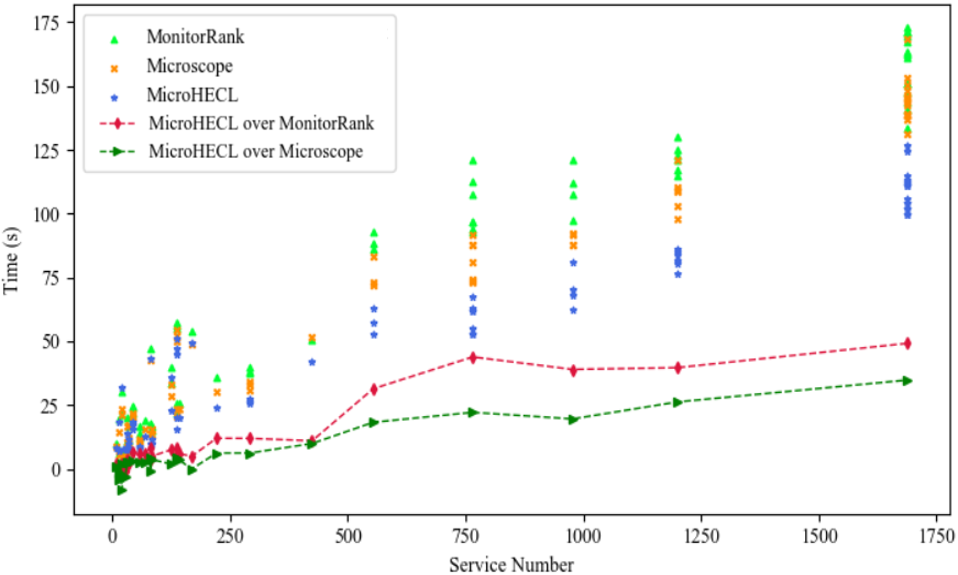
\includegraphics[width=0.5\textwidth]{images/nodes_to_time.png}
	\vspace{-8pt}
	\caption{Detection Time Changes with Num of Nodes}\label{fig:time}
	\vspace{-5pt}
\end{figure}

The advantages of \app~can be explained by its specially designed mechanisms for anomaly propagation analysis.
MonitorRank traverses the service call graph using random walk algorithm and needs to calculate the correlation scores for a large number of the nodes in the graph.
This process is time-consuming when the graph contains many nodes. 
Microscope traverses all the neighboring nodes of an anomalous node, both upstream and downstream.
Moreover, it has no pruning strategy.
In contrast, \app~considers only a single direction (upstream or downstream) for each anomaly type in anomaly propagation chain extension and uses a pruning strategy to eliminate branches that are likely irrelevant to the anomaly propagation.








\subsection{Effect of Pruning (RQ3)}
The pruning strategy is a key for the accuracy and efficiency of root cause localization.
We evaluate the effect of the pruning strategy by analyzing how the accuracy and time of root cause localization change with the threshold of correlation coefficient.
To this end, we run \app~to analyze the 75 availability issues with different threshold settings and measure the accuracy and time.
We choose the top-3 hit ratio (i.e., HR@3) as the indicator of accuracy.

The results of the evaluation are shown in Figure~\ref{fig:rq3}.
It can be seen that both the accuracy and time decrease with the increase of the threshold, as more services and service call edges are pruned in the analysis process and less services are reached and considered.
It can also be seen that the accuracy remains 0.67 when the threshold increases from 0 to 0.7, while the time decreases from 75 seconds to 46 seconds.
This analysis confirms the effectiveness of the pruning strategy, which can significantly improve the efficiency of root cause localization while keeping the accuracy.
And the best threshold is 0.7 for these availability issues.

\begin{figure}[ht]
	\centering
	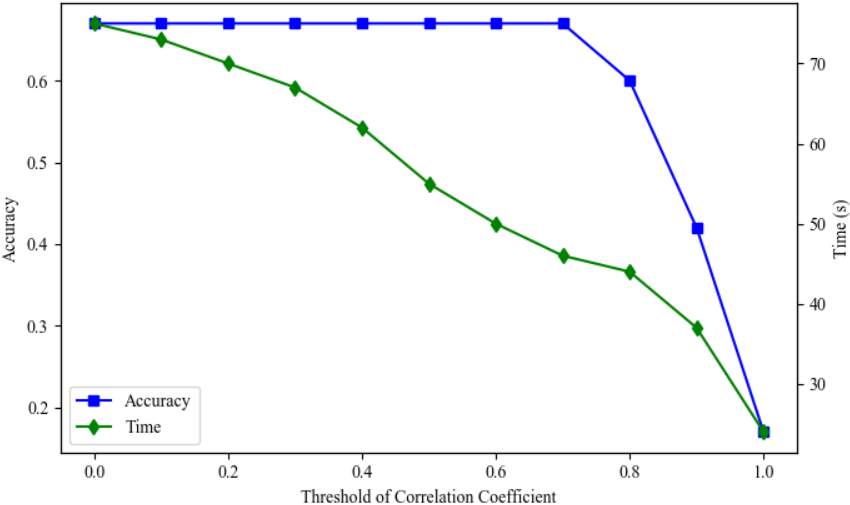
\includegraphics[width=0.5\textwidth]{images/pruningEffect.png}
	\vspace{-8pt}
	\caption{Evaluation of the Effect of the Pruning Strategy}\label{fig:rq3}
	\vspace{-10pt}
\end{figure}



\subsection{Threats to Validity}
A major threat to the internal validity of our studies lies in the implementation of the two baseline approaches.
We implement the two approaches by ourselves based on the descriptions in their papers and thus our implementations may not fully embody the approaches.
Another threat to the internal validity lies in the interactions with the monitoring infrastructure, i.e., EagleEye.
In the experiments, \app~together with the two baseline approaches need to obtain data from EagleEye in real time and there is thus uncertain latency due to limit circuit.
This threat applies to all the three approaches equally.

A major threat to the external validity of our studies lies in the fact that all the studies are conducted with the data and availability issues collected from the e-commerce system of Alibaba.
Microservice systems of other companies or domains may have different characteristics, for example, in the fluctuations of quality metrics and propagation of service anomalies.
The accuracy and efficiency achieved in our studies may not apply to other microservice systems.
